\chapter{Material Anorganik dan Nanomaterial}\label{ch:b3:inorganic-materials}

Sebongkah \omterm{def:b3:inorganic-materials:sol-gel}{aerogel} silika, padatan yang sebagian besar berupa udara, menahan
sekuntum bunga di atas nyala gas tanpa membuatnya layu. \omterm{def:b3:inorganic-materials:sol-gel}{Aerogel} itu adalah
kaca, yang dibuat bukan dengan melelehkan pasir melainkan dengan membiarkan
cairan mengental menjadi \omterm{def:b3:colloids:colloid}{gel} lalu mengeringkan \omterm{def:b3:colloids:colloid}{gel} itu tanpa membiarkannya
runtuh. Kimia material bekerja dengan urutan itu: pilih strukturnya, lalu
rute yang membuatnya, lalu bacalah sifat-sifatnya. Bab ini menelusuri
rute-rute menuju padatan anorganik, struktur \omterm{def:b3:inorganic-materials:ceramic}{keramik}, kaca, dan kristal
berpori, serta apa yang terjadi pada materi ketika sebuah partikel hanya
berukuran beberapa nanometer.

\begin{recall}
Jilid Tahun 1 menjelaskan tipe-tipe struktur kristal, situs interstisial,
alotrop, grafit, dan intan; Jilid Tahun 2 menjelaskan diagram fase, suhu
transisi kaca, dan polimer. \Cref{ch:b3:surfaces-catalysis} mendefinisikan
\omterm{def:b3:surfaces-catalysis:surface-area}{luas permukaan spesifik}, \cref{ch:b3:colloids} \omterm{def:b3:colloids:colloid}{sol} dan \omterm{def:b3:colloids:colloid}{gel},
\cref{ch:b3:solid-state} pita, \omterm{def:b3:solid-state:defects}{cacat titik}, dan \omterm{def:b3:solid-state:ionic-conductor}{konduktor ionik};
\cref{ch:b3:quantum-model-systems} menyelesaikan \omterm{def:b3:quantum-model-systems:box}{partikel dalam kotak}, dan
\cref{ch:b3:point-groups} memberikan grup ikosahedral.
\end{recall}

\begin{omfigure}
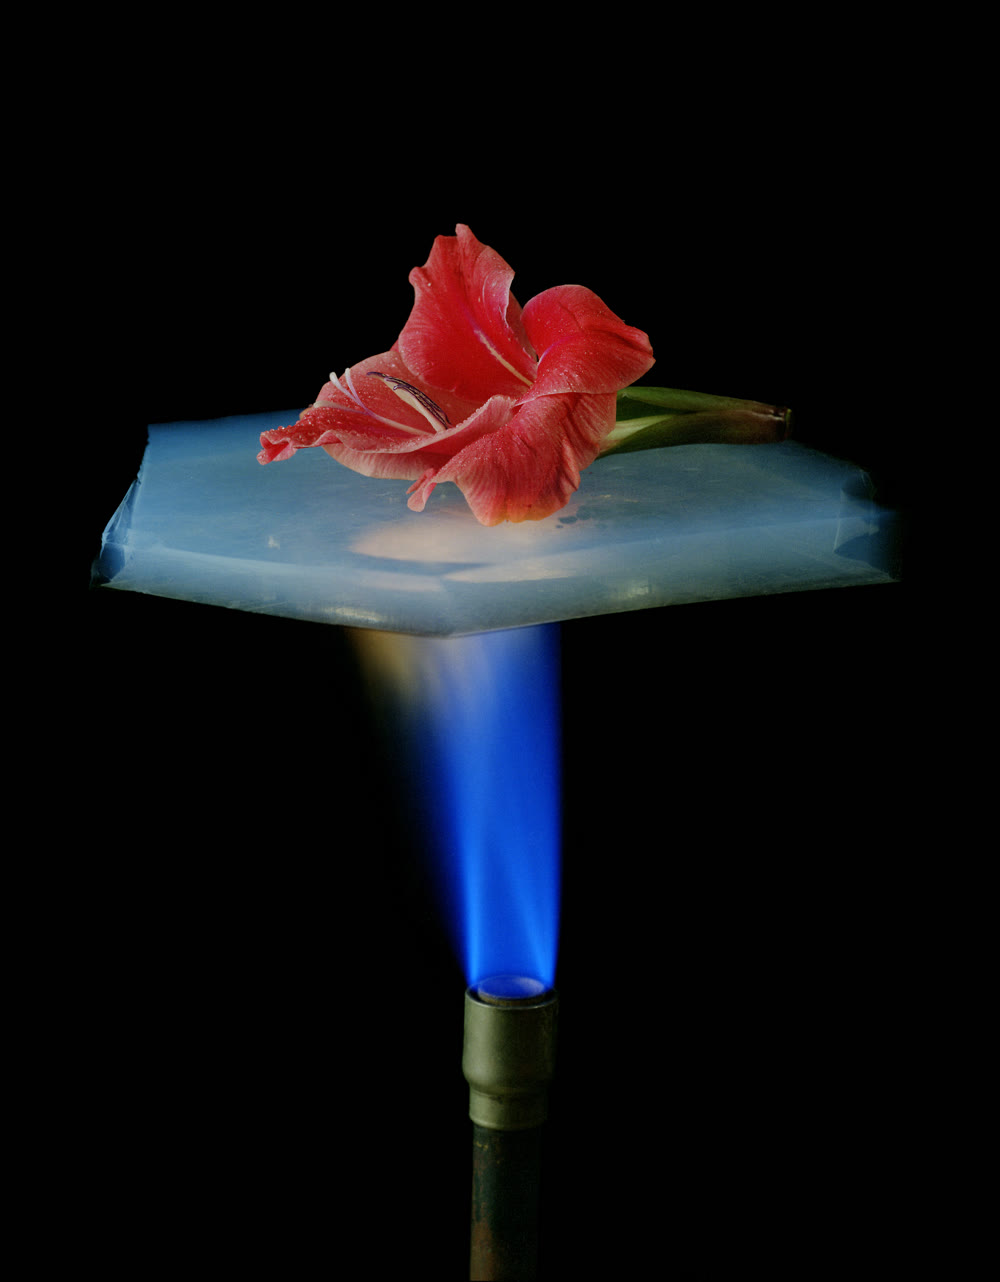
\includegraphics[width=0.38\linewidth]{images/book4/aerogel-flower.jpg}

{\small Sekuntum bunga pada sebongkah \omterm{def:b3:inorganic-materials:sol-gel}{aerogel} silika di atas nyala gas: \omterm{def:b3:inorganic-materials:sol-gel}{aerogel}, yaitu
\omterm{def:b3:colloids:colloid}{gel} kering yang sebagian besar berupa ruang kosong, menghantarkan kalor dengan sangat buruk. Foto:
NASA/JPL, domain publik.}
\end{omfigure}

\section{Rute sintesis}

\begin{definition}[Metode keramik]\label{def:b3:inorganic-materials:ceramic-method}
Yang disebut \emph{metode keramik}\index{metode keramik} adalah cara membuat senyawa padat dengan
menggerus pereaksi-pereaksi padat bersama-sama lalu memanaskannya, sering berhari-hari dan
dengan penggerusan ulang, pada suhu yang cukup tinggi agar ion-ion dapat berdifusi melalui
padatan.
\end{definition}

Reaksi dua padatan terjadi di bidang kontaknya, dan produknya membentuk
lapisan di antara keduanya yang kemudian harus dilalui oleh ion-ion: tahap yang paling lambat
adalah difusi, dan tahap itu makin lambat ketika lapisannya menebal.

\begin{proposition}[Pertumbuhan parabolik]\label{prop:b3:inorganic-materials:parabolic}
Jika pertumbuhan lapisan produk dibatasi oleh difusi melintasinya, tebalnya
tumbuh menurut $x^2 = kt$.
\end{proposition}

\begin{proof}
Dengan konsentrasi yang tetap pada kedua muka lapisan, fluks yang melaluinya
mengikuti hukum Fick, $J = D\Delta c/x$. Lapisan tumbuh sebanding dengan fluks itu:
$\dd x/\dd t = \lambda J = \lambda D\Delta c/x$, dengan $\lambda$ volume produk per mol yang diangkut. Maka
$x\,\dd x = \lambda D\Delta c\,\dd t$, dan integrasi dari $x = 0$ pada $t = 0$ memberikan $x^2 = 2\lambda D\Delta c\,t = kt$.
\end{proof}

Menggandakan ukuran partikel dengan demikian mengalikan waktu reaksi dengan empat: karena itu
dilakukan penggerusan halus, pencampuran pada skala atom dalam sebuah prekursor (\omterm{def:b3:colloids:colloid}{gel} oksalat
atau sitrat campuran yang terurai menjadi senyawa target), atau rute larutan.

\begin{definition}[Proses sol--gel]\label{def:b3:inorganic-materials:sol-gel}
Yang disebut \emph{proses sol--gel}\index{proses sol--gel} adalah cara membuat oksida melalui
hidrolisis dan kondensasi prekursor molekular, biasanya alkoksida, dalam
larutan: larutan itu menjadi \omterm{def:b3:colloids:colloid}{sol} gugusan oksida kecil, lalu \omterm{def:b3:colloids:colloid}{gel}, yaitu
jaringan padat kontinu yang terisi cairan. Jika dikeringkan dengan penguapan, \omterm{def:b3:colloids:colloid}{gel} itu
menyusut menjadi \emph{xerogel}\index{xerogel} yang mampat; jika dikeringkan di atas titik
kritis cairannya, yang menyingkirkan cairan itu tanpa antarmuka cairan--gas, \omterm{def:b3:colloids:colloid}{gel} itu mempertahankan
volumenya sebagai \emph{aerogel}\index{aerogel}.
\end{definition}

\begin{omfigure}
\setchemfig{atom sep=2.0em}
\schemestart
\chemfig{RO-Si(-[2]OR)(-[6]OR)-OR}
\+ \chemfig{H_2O}
\arrow{->[hidrolisis]}[,1.4]
\chemfig{RO-Si(-[2]OR)(-[6]OR)-OH}
\+ ROH
\schemestop
\par\bigskip
\schemestart
\chemfig{{\equiv}Si-OH}
\+
\chemfig{HO-Si{\equiv}}
\arrow{->[kondensasi]}[,1.6]
\chemfig{{\equiv}Si-O-Si{\equiv}}
\+ \chemfig{H_2O}
\schemestop
\par\medskip

{\small Kimia sol--gel sebuah alkoksida silikon (R: gugus alkil, etil dalam
tetraetil ortosilikat): air menggantikan gugus-gugus alkoksi dengan gugus hidroksi, dan
dua silanol berkondensasi menjadi jembatan siloksana. Jika diulang, kondensasi-kondensasi itu membangun
jaringan silika tiga dimensi.}
\end{omfigure}

Kedua reaksi itu bersama-sama memberikan, untuk reaksi yang sempurna,
$\ce{Si(OC2H5)4 + 2H2O -> SiO2 + 4C2H5OH}$. Katalisis asam membuat hidrolisis cepat dan
kondensasi lambat, sehingga terbentuk polimer tipis yang mirip rantai; katalisis basa memberikan
yang sebaliknya, yaitu partikel-partikel mampat. Pelapis (lapisan antipantul pada kaca)
dibuat dengan mencelupkan sebuah benda ke dalam \omterm{def:b3:colloids:colloid}{sol} lalu menariknya keluar.

\begin{definition}[Sintesis hidrotermal]\label{def:b3:inorganic-materials:hydrothermal}
Yang disebut \emph{sintesis hidrotermal}\index{sintesis hidrotermal} adalah cara mengkristalkan
padatan dari air di atas titik didih normalnya, dalam bejana tertutup di bawah tekanan uapnya
sendiri; \emph{sintesis solvotermal}\index{sintesis solvotermal}
melakukan hal yang sama dalam pelarut lain.
\end{definition}

\begin{definition}[Deposisi uap kimia]\label{def:b3:inorganic-materials:cvd}
Yang disebut \emph{deposisi uap kimia}\index{deposisi uap kimia} (CVD) adalah cara menumbuhkan
lapisan padat pada permukaan yang dipanaskan melalui reaksi prekursor-prekursor gas di sana, misalnya
silikon dari silana, $\ce{SiH4 -> Si + 2H2}$, atau intan dari metana dan hidrogen.
\end{definition}

\begin{method}[Memilih rute sintesis]\label{met:b3:inorganic-materials:route}
\begin{enumerate}
  \item Oksida refraktori yang stabil dalam bentuk serbuk ruah: \omterm{def:b3:inorganic-materials:ceramic-method}{metode keramik}, dengan
        prekursor jika pencampurannya sulit.
  \item Fase metastabil, serbuk halus, atau pelapis pada suhu rendah:
        sol--gel atau pengendapan.
  \item Kristal tunggal besar dari fase yang hanya larut dalam air panas (kuarsa) atau
        kerangka yang dibangun di sekitar templat (\omterm{def:b3:inorganic-materials:zeolite}{zeolit}): hidrotermal.
  \item Lapisan tipis yang murni pada substrat (lapisan \omterm{def:b3:solid-state:classes}{semikonduktor}): CVD.
\end{enumerate}
\end{method}

\begin{inthelab}[Pelapis sol--gel dan autoklaf]
Tetraetil ortosilikat diaduk dengan etanol, air, dan setetes asam
sampai larutannya jernih; sebuah kaca preparat yang bersih dicelupkan lalu ditarik keluar dengan
kecepatan lambat yang tetap, dikeringkan, dan dipanaskan, sehingga tertinggal lapisan silika yang cukup tipis untuk
memperlihatkan warna interferensi. Untuk \omterm{def:b3:inorganic-materials:hydrothermal}{sintesis hidrotermal}, pereaksi-pereaksi dimasukkan
ke dalam pelapis dalam dari politetrafluoroetilena, diisi tidak lebih dari sekitar dua pertiga agar
cairan yang memuai tidak memenuhi bejana, ditutup rapat dalam autoklaf
baja, lalu dipanaskan dalam oven; autoklaf baru dibuka setelah dingin.
\end{inthelab}

\begin{omfigure}
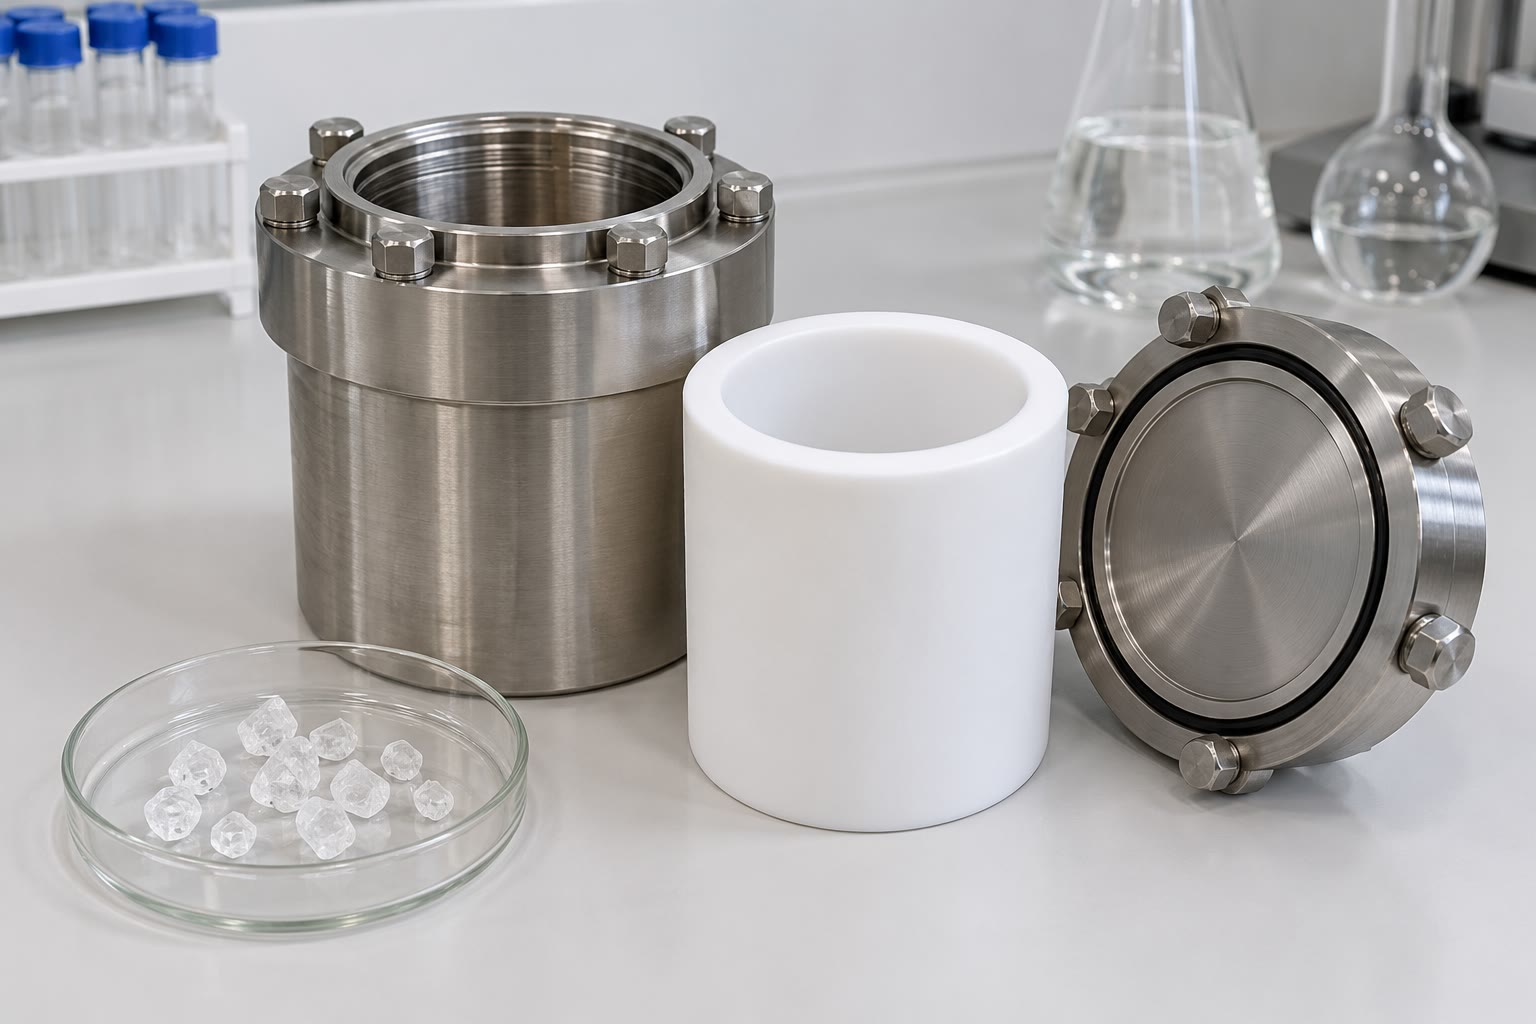
\includegraphics[width=0.5\linewidth]{images/book4/ai/b3-23-autoclave.jpg}

{\small Autoklaf laboratorium untuk \omterm{def:b3:inorganic-materials:hydrothermal}{sintesis hidrotermal}: badan baja dengan
tutup berbaut, pelapis dalam polimer berwarna putih yang menampung campuran reaksi, dan kristal-kristal
yang tumbuh di dalamnya.}
\end{omfigure}

\section{Keramik dan kaca}

\begin{definition}[Keramik]\label{def:b3:inorganic-materials:ceramic}
Yang disebut \emph{keramik}\index{keramik} adalah padatan anorganik nonlogam yang dibuat dengan
memanaskan serbuk: oksida, nitrida, dan karbida, atau produk-produk lempung.
\end{definition}

\begin{definition}[Struktur perovskit]\label{def:b3:inorganic-materials:perovskite}
Yang disebut \emph{struktur perovskit}\index{struktur perovskit} sebuah oksida $\mathrm{ABO_3}$
adalah struktur yang kation-kation B-nya yang kecil terletak di pusat oktahedron $\mathrm{BO_6}$ yang berbagi sudut dan
kation-kation A-nya yang besar berada di rongga berkoordinasi dua belas di antara oktahedron-oktahedron itu; dalam
sel kubus ideal, B berada di pusat, O di pusat-pusat muka, dan A di sudut-sudut.
Yang disebut \emph{faktor toleransi}\index{faktor toleransi} adalah ukuran seberapa baik ion-ion itu
pas:
\[
  t = \frac{r_A + r_O}{\sqrt2\,(r_B + r_O)}.
\]
\end{definition}

\begin{omfigure}
\tdplotsetmaincoords{60}{100}
\begin{tikzpicture}[tdplot_main_coords, scale=1.5, font=\small,
  aA/.style={om atom, ball color=green!45!black, minimum size=7.4mm},
  aB/.style={om atom, ball color=black!35, minimum size=4.4mm},
  aOs/.style={om atom, ball color=red!80, minimum size=4.8mm}]
  \pic[transform shape] {omcubeo={2}};
  % atom-atom dari belakang ke depan untuk pandangan 60/100 (kedalaman 0.853x + 0.150y + 0.5z)
  \node[aA] at (0,0,0) {};
  \node[aA] at (0,2,0) {};
  \node[aOs] (o1) at (0,1,1) {};
  \node[aA] at (0,0,2) {};
  \node[aOs] (o2) at (1,1,0) {};
  \node[aA] at (0,2,2) {};
  \node[aOs] (o3) at (1,0,1) {};
  \node[aB] (b) at (1,1,1) {};
  \node[aOs] (o4) at (1,2,1) {};
  \node[aA] at (2,0,0) {};
  \node[aOs] (o5) at (1,1,2) {};
  \node[aA] at (2,2,0) {};
  \node[aOs] (o6) at (2,1,1) {};
  \node[aA] at (2,0,2) {};
  \node[aA] at (2,2,2) {};
  \begin{scope}[on background layer]
    \draw[omMeth!70, line width=0.6pt] (o1.center) -- (o2.center) -- (o6.center) -- (o5.center) -- cycle
      (o3.center) -- (o2.center) -- (o4.center) -- (o5.center) -- cycle
      (o1.center) -- (o3.center) -- (o6.center) -- (o4.center) -- cycle;
    \draw[bond] (b.center) -- (o1.center) (b.center) -- (o2.center) (b.center) -- (o3.center)
      (b.center) -- (o4.center) (b.center) -- (o5.center) (b.center) -- (o6.center);
  \end{scope}
  \node[anchor=west] at (2,3.35,2) {A};
  \node[anchor=west] at (2,3.35,1) {O};
  \node[anchor=west] at (2,3.35,0) {B};
  \node[aA, minimum size=4mm] at (2,3.2,2) {};
  \node[aOs, minimum size=3.2mm] at (2,3.2,1) {};
  \node[aB, minimum size=3mm] at (2,3.2,0) {};
\end{tikzpicture}

{\small Sel perovskit kubus $\mathrm{ABO_3}$: kation B (abu-abu) di pusat
oktahedron enam ion oksida di pusat-pusat muka (rusuk hijau), dan kation-kation A
di sudut-sudut. Setiap ion A di sudut dimiliki bersama oleh delapan sel dan setiap oksigen oleh
dua sel: satu A, satu B, dan tiga O per sel.}
\end{omfigure}

\begin{proposition}[Faktor toleransi ideal]\label{prop:b3:inorganic-materials:tolerance}
Dalam perovskit kubus ideal, dengan ion-ion yang bersentuhan sepanjang arah B--O dan A--O,
$t = 1$.
\end{proposition}

\begin{proof}
Dengan rusuk $a$, B di pusat dan O di pusat muka berjarak $a/2$: $r_B + r_O = a/2$.
A di sudut dan O di pusat muka yang berdampingan berjarak setengah diagonal muka:
$r_A + r_O = a\sqrt2/2$. Dengan membagi, $(r_A + r_O)/(r_B + r_O) = \sqrt2$, sehingga $t = 1$.
\end{proof}

Jika $t$ sedikit di bawah 1, ion A terlalu kecil untuk rongganya dan
oktahedron-oktahedron itu miring untuk merapat di sekelilingnya, sehingga simetrinya turun; jika $t$ di atas 1,
ion B terlalu kecil untuk oktahedronnya dan dapat bergeser dari pusat.

\begin{definition}[Feroelektrik]\label{def:b3:inorganic-materials:ferroelectric}
Yang disebut \emph{feroelektrik}\index{feroelektrik} adalah kristal dengan polarisasi listrik
spontan yang dapat dibalik oleh medan listrik yang diberikan.
\end{definition}

% ledger: rion:Ba2+XII, rion:Ti4+VI, rion:O2-VI
Barium titanat adalah contoh klasiknya: dengan $r(\ce{Ba^2+}) = \qty{161}{pm}$ (berkoordinasi dua belas),
$r(\ce{Ti^4+}) = \qty{60.5}{pm}$, dan $r(\ce{O^2-}) = \qty{140}{pm}$, $t = 1.06$. Di bawah sebuah suhu transisi, ion-ion
titanium bergeser dari pusat, semuanya ke arah yang sama di dalam satu domain,
dan kristalnya terpolarisasi; permitivitas yang sangat besar di dekat transisi membuat
barium titanat menjadi dielektrik sebagian besar kapasitor \omterm{def:b3:inorganic-materials:ceramic}{keramik}.

\begin{definition}[Kaca oksida]\label{def:b3:inorganic-materials:glass}
Yang disebut \emph{kaca oksida}\index{kaca oksida} adalah padatan oksida amorf, yang dibuat dengan
mendinginkan lelehan tanpa kristalisasi. Yang disebut \emph{pembentuk
jaringan}\index{pembentuk jaringan} ($\ce{SiO2}$, $\ce{B2O3}$, $\ce{P2O5}$) adalah oksida yang membangun jaringan kontinu
polihedron yang berbagi sudut; sedangkan \emph{pengubah jaringan}\index{pengubah jaringan}
($\ce{Na2O}$, $\ce{CaO}$) memutus jembatan-jembatan dalam jaringan itu, dan setiap ion oksida yang ditambahkan mengubah satu
oksigen penjembatan menjadi dua oksigen bukan penjembatan, dengan kation-kationnya menempati
rongga-rongga.
\end{definition}

\begin{omfigure}
\begin{tikzpicture}
\begin{axis}[name=c, width=0.5\linewidth, axis equal image, hide axis, xmin=-1.2, xmax=12.6, ymin=-1.2, ymax=8.7]
\addplot[quiver={u=\thisrow{u}, v=\thisrow{v}}, -, black!60, line width=0.6pt] table {figdata/out/bachelor-3-glass-network-crystal-bonds.dat};
\addplot[only marks, mark=*, mark size=2.2pt, omDef] table {figdata/out/bachelor-3-glass-network-crystal-T.dat};
\addplot[only marks, mark=*, mark size=1.3pt, omThm, mark options={fill=white}] table {figdata/out/bachelor-3-glass-network-crystal-O.dat};
\end{axis}
\begin{axis}[at={(c.east)}, anchor=west, xshift=0.2cm, width=0.5\linewidth, axis equal image, hide axis, xmin=-1.2, xmax=12.6, ymin=-1.2, ymax=8.7]
\addplot[quiver={u=\thisrow{u}, v=\thisrow{v}}, -, black!60, line width=0.6pt] table {figdata/out/bachelor-3-glass-network-glass-bonds.dat};
\addplot[only marks, mark=*, mark size=2.2pt, omDef] table {figdata/out/bachelor-3-glass-network-glass-T.dat};
\addplot[only marks, mark=*, mark size=1.3pt, omThm, mark options={fill=white}] table {figdata/out/bachelor-3-glass-network-glass-O.dat};
\addplot[only marks, mark=*, mark size=1.5pt, omThm] table {figdata/out/bachelor-3-glass-network-glass-NBO.dat};
\addplot[only marks, mark=*, mark size=2.6pt, omProp] table {figdata/out/bachelor-3-glass-network-glass-Na.dat};
\end{axis}
\end{tikzpicture}

{\small Gambaran dua dimensi sebuah kristal dan sebuah kaca dengan komposisi
yang sama (biru: pembentuk berkoordinasi tiga; lingkaran merah terbuka: oksigen
penjembatan). Kiri, kristal mengulang satu cincin. Kanan, kaca: setiap pembentuk
masih memiliki tiga oksigen pada jarak yang hampir sama, tetapi cincin-cincinnya beranggota lima,
enam, atau tujuh dan tidak ada yang berulang; di dua tempat, sebuah pengubah telah memutus sebuah
jembatan, sehingga tertinggal dua oksigen bukan penjembatan (merah terisi) dan sebuah kation (jingga) di dalam
rongga. Jaringan model, yang direlaksasi dengan pegas.}
\end{omfigure}

Pada 1932 William Zachariasen berargumen bahwa sebuah oksida mudah membentuk kaca jika
kationnya dikelilingi oleh sedikit oksigen (tiga atau empat), setiap oksigen menghubungkan paling banyak
dua kation, dan polihedron-polihedronnya berbagi sudut, bukan rusuk atau muka: maka
jaringan acak hanya memerlukan sedikit lebih banyak energi daripada kristalnya. Kaca jendela adalah
silika dengan natrium oksida dan kalsium oksida sebagai pengubah, yang menurunkan suhu
leleh. Kaca penutup ponsel yang diperkuat direndam dalam kalium nitrat
cair: ion $\ce{K+}$ yang lebih besar menggantikan ion $\ce{Na+}$ di permukaan dan, karena berdesakan,
menempatkan permukaan itu di bawah tekanan, sehingga retakan tidak dapat membuka.

\section{Padatan berpori: zeolit dan kerangka}

\begin{definition}[Zeolit]\label{def:b3:inorganic-materials:zeolite}
Yang disebut \emph{zeolit}\index{zeolit} adalah aluminosilikat kristalin yang
kerangka tetrahedron $\ce{SiO4}$ dan $\ce{AlO4}$-nya yang berbagi sudut melingkupi sangkar dan
saluran berukuran molekul, dengan kation yang dapat dipertukarkan dan air di dalamnya. Yang disebut
\emph{ayakan molekul}\index{ayakan molekul} adalah padatan berpori yang menerima
molekul menurut ukurannya; sedangkan \emph{selektivitas bentuk}\index{selektivitas bentuk}
adalah pengendalian sebuah reaksi oleh ukuran dan bentuk pori-pori tempat
reaksi itu berlangsung.
\end{definition}

Setiap tetrahedron $\ce{AlO4}$ membawa satu muatan negatif lebih banyak daripada $\ce{SiO4}$
(aluminium(III) menggantikan silikon(IV)); kation-kation di dalam sangkar, $\ce{Na+}$ atau $\ce{Ca^2+}$,
mengimbanginya, dan dapat dipertukarkan.

\begin{proposition}[Aturan Löwenstein]\label{prop:b3:inorganic-materials:lowenstein}
Dalam kerangka \omterm{def:b3:inorganic-materials:zeolite}{zeolit}, dua tetrahedron $\ce{AlO4}$ tidak pernah berbagi oksigen: tautan Al--O--Al
tidak ada (sebuah pengamatan pada semua kerangka aluminosilikat yang dikenal). Akibatnya,
rasio Si/Al sebuah \omterm{def:b3:inorganic-materials:zeolite}{zeolit} paling kecil 1.
\end{proposition}

\begin{proof}[Bukti akibatnya]
Setiap aluminium memiliki empat oksigen, yang masing-masing menurut aturan itu dimiliki bersama dengan sebuah silikon:
$4N_{\mathrm{Al}}$ tautan Al--O--Si. Setiap silikon hanya memiliki empat oksigen, sehingga ikut dalam
paling banyak empat tautan semacam itu: $4N_{\mathrm{Al}} \le 4N_{\mathrm{Si}}$, yaitu $N_{\mathrm{Si}}/N_{\mathrm{Al}} \ge 1$. Kesamaan memaksa setiap
silikon memiliki empat tetangga aluminium: Si dan Al berselang-seling.
\end{proof}

\begin{omfigure}
\tdplotsetmaincoords{55}{135}
\begin{tikzpicture}[tdplot_main_coords, scale=0.85, font=\small, baseline=(current bounding box.center),
  tSi/.style={circle, inner sep=0pt, minimum size=2.6mm, draw=black!70, fill=omDef!80},
  tAl/.style={circle, inner sep=0pt, minimum size=2.6mm, draw=black!70, fill=omProp!80}]
  % rusuk-rusuk oktahedron terpancung (titik sudut: permutasi (0, +-1, +-2));
  % rusuk tersembunyi (kedua mukanya membelakangi pandangan ini) putus-putus
  \foreach \a/\b/\c/\d/\e/\f in {-2/-1/0/-2/0/-1, -2/-1/0/-2/0/1, -2/-1/0/-1/-2/0, -2/0/-1/-2/1/0, -2/0/-1/-1/0/-2, -1/-2/0/0/-2/-1, -1/-2/0/0/-2/1, -1/0/-2/0/-1/-2, -1/0/-2/0/1/-2, 0/-2/-1/0/-1/-2, 0/-2/-1/1/-2/0, 0/-1/-2/1/0/-2}
    \draw[black!40, dashed] (\a,\b,\c) -- (\d,\e,\f);
  \foreach \a/\b/\c/\d/\e/\f in {-2/0/1/-2/1/0, -2/0/1/-1/0/2, -2/1/0/-1/2/0, -1/0/2/0/-1/2, -1/0/2/0/1/2, -1/2/0/0/2/-1, -1/2/0/0/2/1, 0/-2/1/0/-1/2, 0/-2/1/1/-2/0, 0/-1/2/1/0/2, 0/1/-2/0/2/-1, 0/1/-2/1/0/-2, 0/1/2/0/2/1, 0/1/2/1/0/2, 0/2/-1/1/2/0, 0/2/1/1/2/0, 1/-2/0/2/-1/0, 1/0/-2/2/0/-1, 1/0/2/2/0/1, 1/2/0/2/1/0, 2/-1/0/2/0/-1, 2/-1/0/2/0/1, 2/0/-1/2/1/0, 2/0/1/2/1/0}
    \draw[black!75, line width=0.7pt] (\a,\b,\c) -- (\d,\e,\f);
  % atom T dari belakang ke depan; yang tersembunyi lebih pucat
  \foreach \x/\y/\z/\k/\v in {-2/-1/0/Si/0, -1/-2/0/Al/0, -2/0/-1/Al/0, 0/-2/-1/Si/0, -1/0/-2/Si/0, 0/-1/-2/Al/0, -2/0/1/Al/1, 0/-2/1/Si/1, -2/1/0/Si/1, 1/-2/0/Al/1, 0/1/-2/Al/1, 1/0/-2/Si/1, -1/0/2/Si/1, 0/-1/2/Al/1, -1/2/0/Al/1, 2/-1/0/Si/1, 0/2/-1/Si/1, 2/0/-1/Al/1, 0/1/2/Al/1, 1/0/2/Si/1, 0/2/1/Si/1, 2/0/1/Al/1, 1/2/0/Al/1, 2/1/0/Si/1}
    \node[t\k, opacity=0.35+0.65*\v] at (\x,\y,\z) {};
\end{tikzpicture}
\hspace{1.2cm}
\begin{tikzpicture}[font=\small, scale=0.8, baseline=(current bounding box.center)]
  \foreach \i in {0,1,2} \foreach \j in {0,1,2} {
    \fill[omDef!70] ($(2.2*\i,2.2*\j)+(-0.28,-0.28)$) rectangle +(0.56,0.56);
  }
  \foreach \i in {0,1} \foreach \j in {0,1,2} {
    \draw[black!70, line width=0.8pt] (2.2*\i+0.28,2.2*\j) -- (2.2*\i+0.75,2.2*\j);
    \draw[black!70, line width=0.8pt] (2.2*\i+1.45,2.2*\j) -- (2.2*\i+1.92,2.2*\j);
    \node[draw=black!70, regular polygon, regular polygon sides=6, minimum size=5.6mm, inner sep=0pt] at (2.2*\i+1.1,2.2*\j) {};
  }
  \foreach \i in {0,1,2} \foreach \j in {0,1} {
    \draw[black!70, line width=0.8pt] (2.2*\i,2.2*\j+0.28) -- (2.2*\i,2.2*\j+0.75);
    \draw[black!70, line width=0.8pt] (2.2*\i,2.2*\j+1.45) -- (2.2*\i,2.2*\j+1.92);
    \node[draw=black!70, regular polygon, regular polygon sides=6, minimum size=5.6mm, inner sep=0pt] at (2.2*\i,2.2*\j+1.1) {};
  }
  \node[font=\scriptsize, align=center] at (1.1,-0.85) {simpul $\ce{Zn4O}$ $+$ penaut tereftalat};
\end{tikzpicture}

{\small Kiri: sangkar sodalit, satuan bangun \omterm{def:b3:inorganic-materials:zeolite}{zeolit} A, dengan atom
tetrahedral di setiap sudut (oksigen, di tengah setiap rusuk, tidak
digambar); silikon (biru) dan aluminium (jingga) berselang-seling, seperti yang dituntut aturan Löwenstein
jika Si/Al = 1. Kanan: satu lapisan \omterm{def:b3:inorganic-materials:mof}{kerangka logam--organik},
skematis: gugusan $\ce{Zn4O}$ (persegi) yang dihubungkan oleh penaut benzena-1,4-dikarboksilat
(cincin) menjadi kisi kubus dengan pori-pori besar.}
\end{omfigure}

\begin{method}[Rumus dan kapasitas tukar sebuah zeolit]\label{met:b3:inorganic-materials:zeolite-formula}
\begin{enumerate}
  \item Tuliskan kerangkanya sebagai $\mathrm{[(AlO_2)_x(SiO_2)_y]^{x-}}$: Si/Al $= y/x$.
  \item Muatan kerangka $-x$ diimbangi oleh kation: $x$ kation monovalen atau $x/2$ kation
        divalen.
  \item Kapasitas tukar adalah jumlah muatan yang dapat dipertukarkan per gram:
        $x/M$ mol kation monovalen, $x/2M$ mol kation divalen, dengan $M$
        massa molar rumus sebagaimana ditimbang (anhidrat atau terhidrat).
\end{enumerate}
\end{method}

\begin{proposition}[Kapasitas tukar]\label{prop:b3:inorganic-materials:exchange-capacity}
Kapasitas sebuah \omterm{def:b3:inorganic-materials:zeolite}{zeolit} untuk kation bermuatan $z$ adalah $x/(zM)$ mol per gram,
dengan $x$ jumlah atom aluminium dalam rumus yang massa molarnya $M$.
\end{proposition}

\begin{proof}
Setiap aluminium menyumbang satu muatan negatif pada kerangka; kenetralan listrik
mensyaratkan $x$ satuan muatan positif, yang semuanya dapat dipertukarkan, sehingga
terdapat $x/z$ kation bermuatan $z$ per satuan rumus, yaitu per massa $M$.
\end{proof}

% ledger: iza:LTA.window, iza:MFI.channels
\omterm{def:b3:inorganic-materials:zeolite}{Zeolit} A memiliki jendela dari delapan tetrahedron, selebar \qty{0.41}{nm}: air dan ion-ion
kecil dapat lewat, molekul bercabang tidak. ZSM-5 memiliki dua himpunan saluran dari sepuluh
tetrahedron, sekitar 0.51 sampai \qty{0.56}{nm}: dalam konversi metanol atau
alkilasi toluena, \textit{para}-xilena yang ramping berdifusi keluar jauh lebih cepat daripada
isomer \textit{orto} dan \textit{meta}-nya, yang tetap tinggal dan berisomerisasi. Itulah \omterm{def:b3:inorganic-materials:zeolite}{selektivitas
bentuk}.

\begin{definition}[Kerangka logam--organik]\label{def:b3:inorganic-materials:mof}
Yang disebut \emph{kerangka logam--organik}\index{kerangka logam--organik} (MOF) adalah
padatan kristalin yang dibangun dari ion atau gugusan logam yang dihubungkan oleh penaut
organik politopik menjadi jaringan berpori. Yang disebut \emph{satuan bangun
sekunder}\index{satuan bangun sekunder} adalah gugusan logam beserta gugus-gugus
koordinasinya, yang diperlakukan sebagai satu simpul jaringan; sedangkan \emph{sintesis
retikular}\index{sintesis retikular} adalah perancangan kerangka dengan memilih
simpul dan penaut yang geometrinya tertentu sehingga keduanya tersusun menjadi jaringan yang dipilih.
\end{definition}

% ledger: cod:MOF5.formula, cod:MOF5.a
Dalam MOF-5, gugusan $\ce{Zn4O}$ dengan enam gugus karboksilat merupakan simpul oktahedral,
dan penaut benzena-1,4-dikarboksilat menghubungkannya sepanjang rusuk-rusuk jaringan
kubus, $a = \qty{25.82}{\angstrom}$ untuk sel dengan delapan simpul. Mengganti penautnya dengan penaut yang lebih
panjang mempertahankan jaringannya dan memperbesar pori-porinya: itulah gagasan retikular. Kerangka
semacam itu memiliki luas permukaan ribuan meter persegi per gram dan sedang
diteliti untuk menyimpan hidrogen dan metana serta untuk menangkap karbon dioksida.

\begin{definition}[Ukuran pori]\label{def:b3:inorganic-materials:pores}
% ledger: pore:micro, pore:macro
Menurut konvensi, \emph{mikropori}\index{mikropori} lebih sempit daripada \qty{2}{nm},
\emph{mesopori}\index{mesopori} berukuran antara 2 dan \qty{50}{nm}, dan
\emph{makropori}\index{makropori} lebih lebar daripada \qty{50}{nm}.
\end{definition}

\omterm{def:b3:inorganic-materials:zeolite}{Zeolit} dan sebagian besar MOF bersifat \omterm{def:b3:inorganic-materials:pores}{mikropori}; \omterm{def:b3:colloids:colloid}{gel} silika dan \omterm{def:b3:inorganic-materials:sol-gel}{aerogel} bersifat \omterm{def:b3:inorganic-materials:pores}{mesopori}.

\section{Nanopartikel}

\begin{definition}[Nanomaterial]\label{def:b3:inorganic-materials:nano}
Yang disebut \emph{nanomaterial}\index{nanomaterial} adalah bahan yang paling sedikit satu dimensinya berukuran antara
sekitar 1 dan \qty{100}{nm}; sedangkan \emph{nanopartikel}\index{nanopartikel} memiliki ketiga
dimensinya dalam rentang itu.
\end{definition}

\begin{proposition}[Gugusan ajaib]\label{prop:b3:inorganic-materials:magic}
Gugusan kuboktahedral yang terdiri atas sebuah atom pusat dan $n$ kulit lengkap memiliki
\[
  N(n) = \frac{10n^3 + 15n^2 + 11n + 3}{3}
\]
atom, dan $10n^2 + 2$ di antaranya berada di permukaan: 13, 55, 147, 309, \dots
\end{proposition}

\begin{proof}
Kulit ke-$k$ sebuah kuboktahedron memiliki 12 titik sudut, 24 rusuk yang masing-masing memuat $k - 1$ atom
di dalamnya, 8 muka segitiga yang masing-masing memuat $(k - 1)(k - 2)/2$ atom dalam, dan 6
muka persegi dengan $(k - 1)^2$: totalnya $12 + 24(k - 1) + 4(k - 1)(k - 2) + 6(k - 1)^2 = 10k^2 + 2$. Maka
$N(n) = 1 + \sum_{k=1}^{n}(10k^2 + 2) = 1 + \frac{10n(n + 1)(2n + 1)}{6} + 2n$, yang jika dijabarkan memberikan rumus itu; kulit
terluar, $10n^2 + 2$ atom, adalah permukaannya.
\end{proof}

\begin{omfigure}
\begin{tikzpicture}
\begin{axis}[name=a, width=0.47\linewidth, height=5.4cm, xmin=0, xmax=18, ymin=0, ymax=1,
  axis lines=left, xlabel={diameter / \unit{nm}}, ylabel={fraksi atom di permukaan},
  tick label style={font=\scriptsize}, label style={font=\small}]
\addplot[omDef, thick, mark=*, mark size=1pt] table[x=diam_nm, y=fsurf] {figdata/out/bachelor-3-nanoparticle-size.dat};
\end{axis}
\begin{axis}[at={(a.east)}, anchor=west, xshift=1.5cm, width=0.47\linewidth, height=5.4cm,
  xmin=0.8, xmax=6, ymin=0, ymax=3, axis lines=left,
  xlabel={jari-jari $R$ / \unit{nm}}, ylabel={energi kurungan / \unit{eV}},
  tick label style={font=\scriptsize}, label style={font=\small}]
\addplot[omThm, thick] table[x=R_nm, y=dE_eV] {figdata/out/bachelor-3-nanoparticle-size-b.dat};
\end{axis}
\end{tikzpicture}

{\small Kiri: fraksi atom di permukaan gugusan emas kuboktahedral
terhadap diameternya: lebih dari setengah untuk gugusan yang lebih kecil daripada sekitar
\qty{3}{nm}, dan masih seperlima pada \qty{8}{nm}. Kanan: energi kurungan sepasang
elektron--lubang dalam \omterm{def:b3:inorganic-materials:quantum-dot}{titik kuantum} bulat (\omterm{def:b3:quantum-model-systems:oscillator}{massa tereduksi} model $0.10\,m_e$),
yang menambah \omterm{def:b3:solid-state:band}{celah pita} dan turun sebanding dengan $1/R^2$.}
\end{omfigure}

Karena sebagian besar atomnya berada di permukaan, tempat atom-atom itu memiliki lebih sedikit
tetangga, sebuah \omterm{def:b3:inorganic-materials:nano}{nanopartikel} meleleh pada suhu yang lebih rendah daripada logam ruahnya,
lebih reaktif, dan dapat menjadi katalis yang jauh lebih baik: emas ruah bersifat inert, sedangkan
partikel emas berukuran beberapa nanometer mengoksidasi karbon monoksida pada suhu kamar.

\begin{definition}[Titik kuantum]\label{def:b3:inorganic-materials:quantum-dot}
Yang disebut \emph{titik kuantum}\index{titik kuantum} adalah nanokristal \omterm{def:b3:solid-state:classes}{semikonduktor} yang cukup kecil
sehingga kurungan elektron dan \omterm{def:b3:solid-state:carriers}{lubangnya} menaikkan \omterm{def:b3:solid-state:band}{celah pitanya}
di atas \omterm{def:b3:solid-state:band}{celah pita} padatan ruahnya.
\end{definition}

\begin{theorem}[Kurungan dalam bola]\label{thm:b3:inorganic-materials:quantum-dot}
Partikel bermassa $m$ yang terkurung dalam bola berjari-jari $R$ oleh dinding tak hingga memiliki
energi keadaan dasar $E = \hbar^2\pi^2/(2mR^2) = h^2/(8mR^2)$, dengan fungsi gelombang $\psi \propto \sin(\pi r/R)/r$.
\end{theorem}

\begin{proof}
Untuk keadaan yang simetris bola $\psi(r) = u(r)/r$, \omterm{def:b3:quantum-model-systems:operator}{operator} Laplace memberikan
$\nabla^2\psi = u''/r$, sehingga \omterm{thm:b3:quantum-model-systems:schrodinger}{persamaan Schrödinger} di dalam bola menjadi $-\frac{\hbar^2}{2m}u'' = Eu$, yaitu persamaan partikel pada
garis. Solusi dengan $\psi$ yang terhingga di pusat memiliki $u(0) = 0$: $u = \sin(kr)$, dengan $E = \hbar^2k^2/2m$.
Dinding mensyaratkan $u(R) = 0$, sehingga $kR = \pi$ untuk keadaan dasar, dan $E = \hbar^2\pi^2/(2mR^2)$.
\end{proof}

Dalam \omterm{def:b3:inorganic-materials:quantum-dot}{titik kuantum}, elektron dan \omterm{def:b3:solid-state:carriers}{lubang} sama-sama terkurung; energi
eksitasi terendahnya adalah $E_g + h^2/(8\mu R^2)$ dalam pendekatan pertama, dengan $\mu$ \omterm{def:b3:quantum-model-systems:oscillator}{massa tereduksi}
keduanya (tarikan Coulomb di antara keduanya sedikit menurunkannya). Mengurangi jari-jari menjadi setengahnya
mengalikan energi kurungan dengan empat: \omterm{def:b3:inorganic-materials:quantum-dot}{titik kuantum} kadmium selenida berukuran beberapa
nanometer berpendar merah, hijau, atau biru hanya menurut ukurannya, dan dipakai sebagai
pemancar dalam layar.

\begin{definition}[Resonansi plasmon permukaan]\label{def:b3:inorganic-materials:plasmon}
Yang disebut \emph{resonansi plasmon permukaan}\index{resonansi plasmon permukaan} adalah
osilasi kolektif elektron-elektron konduksi sebuah \omterm{def:b3:inorganic-materials:nano}{nanopartikel} logam yang
digerakkan oleh cahaya; resonansi itu memberikan pita serapan yang kuat, yang panjang gelombangnya bergantung pada
logam, ukuran dan bentuk partikel, serta lingkungannya.
\end{definition}

\omterm{def:b3:inorganic-materials:nano}{Nanopartikel} emas berukuran beberapa puluh nanometer menyerap cahaya hijau dan tampak
merah delima dalam kaca atau \omterm{def:b3:colloids:colloid}{koloid}; ketika partikel-partikel itu beragregasi, pitanya bergeser ke panjang
gelombang yang lebih besar dan warnanya menjadi biru: inilah dasar banyak tes cepat, tempat
\omterm{def:b3:colloids:colloid}{koloid} emas yang dilapisi antibodi berkumpul menjadi sebuah garis berwarna.

\section{Nanomaterial karbon}

\begin{definition}[Nanomaterial karbon]\label{def:b3:inorganic-materials:carbon}
Yang disebut \emph{fulerena}\index{fulerena} adalah molekul sangkar tertutup dari atom-atom karbon,
yang masing-masing terikat pada tiga atom lainnya, dengan cincin beranggota lima dan enam, seperti
$\ce{C60}$ yang ikosahedral. Yang disebut \emph{nanotabung karbon}\index{nanotabung karbon} adalah lembaran
grafit yang digulung menjadi silinder tanpa sambungan yang berdiameter sekitar satu nanometer.
Yang disebut \emph{grafena}\index{grafena} adalah satu lapisan grafit setebal satu atom.
\end{definition}

\begin{proposition}[Dua belas segi lima]\label{prop:b3:inorganic-materials:euler}
Setiap \omterm{def:b3:inorganic-materials:carbon}{fulerena} memiliki tepat dua belas segi lima, berapa pun jumlah
segi enamnya.
\end{proposition}

\begin{proof}
Sangkar tertutup adalah sebuah polihedron: rumus Euler $V - E + F = 2$ berlaku. Setiap atom memiliki
tiga ikatan dan setiap ikatan dua atom: $2E = 3V$. Dengan $p$ segi lima dan $h$ segi enam,
penghitungan rusuk melalui muka memberikan $2E = 5p + 6h$, dan $F = p + h$. Maka $V = 2E/3$ dan rumus
Euler menjadi $-E/3 + p + h = 2$, yaitu $-(5p + 6h)/6 + p + h = 2$, sehingga $p/6 = 2$: $p = 12$.
\end{proof}

\begin{omfigure}
\begin{tikzpicture}[scale=0.62, font=\small]
  \def\hexd{0.6}
  \begin{scope}
    \clip (-0.4,-0.5) rectangle (9.6,5.2);
    \foreach \i in {-3,...,10} \foreach \j in {-1,...,6} {
      \pgfmathsetmacro\cx{1.7320508*\hexd*(\i + 0.5*\j)}
      \pgfmathsetmacro\cy{1.5*\hexd*\j}
      \draw[black!45] ({\cx+\hexd*cos(30)},{\cy+\hexd*sin(30)})
        \foreach \k in {90,150,...,390} { -- ({\cx+\hexd*cos(\k)},{\cy+\hexd*sin(\k)}) };
    }
  \end{scope}
  \draw[->, thick, omDef] (0,0) -- ({1.7320508*\hexd},0) node[below right, font=\scriptsize, fill=white, inner sep=1pt] {$\mathbf a_1$};
  \draw[->, thick, omDef] (0,0) -- ({1.7320508*\hexd*0.5},{1.5*\hexd}) node[left, font=\scriptsize, fill=white, inner sep=1pt] {$\mathbf a_2$};
  \draw[->, very thick, omThm] (0,0) -- ({1.7320508*\hexd*(4+0.5*2)},{1.5*\hexd*2}) node[above right, font=\scriptsize, fill=white, inner sep=1pt] {$\mathbf C_h = 4\mathbf a_1 + 2\mathbf a_2$};
  \draw[dashed, omMeth, thick] (0,0) -- ({1.7320508*\hexd*9},0) node[right, font=\scriptsize] {zigzag $(n, 0)$};
  \draw[dashed, omProp, thick] (0,0) -- ({1.7320508*\hexd*5*1.5},{1.5*\hexd*5}) node[below right, font=\scriptsize, fill=white, inner sep=1pt] {kursi $(n, n)$};
\end{tikzpicture}

{\small Lembaran \omterm{def:b3:inorganic-materials:carbon}{grafena} dan vektor kiral sebuah nanotabung: menggulung lembaran itu
sehingga ujung $\mathbf C_h = n\mathbf a_1 + m\mathbf a_2$ bertemu dengan titik asalnya memberikan tabung $(n, m)$, di sini $(4, 2)$.
Sepanjang $\mathbf a_1$, tepi tabung $(n, 0)$ berbentuk zigzag; sepanjang $\mathbf a_1 + \mathbf a_2$, pada 30°, tepi tabung $(n, n)$
berbentuk kursi.}
\end{omfigure}

\begin{proposition}[Nanotabung logam dan semikonduktor]\label{prop:b3:inorganic-materials:nanotube}
\omterm{def:b3:inorganic-materials:carbon}{Nanotabung karbon} berdinding tunggal $(n, m)$ bersifat logam jika $n - m$ kelipatan 3, dan
bersifat \omterm{def:b3:solid-state:classes}{semikonduktor} jika tidak. \admitted
\end{proposition}

Jadi sepertiga dari semua tabung yang mungkin bersifat logam, termasuk setiap tabung
kursi; celah tabung-tabung lainnya mengecil ketika diameternya bertambah. \omterm{def:b3:inorganic-materials:carbon}{Grafena} sendiri
sama sekali tidak memiliki celah: \omterm{def:b3:solid-state:band}{pita valensi} dan \omterm{def:b3:solid-state:band}{pita konduksinya} bersentuhan di titik-titik tunggal, dan
elektron-elektronnya bergerak seolah-olah tidak bermassa.

\begin{safety}{\ghs[0.62cm]{GHS02}\ghs[0.62cm]{GHS07}\ghs[0.62cm]{GHS08}}
% ledger: ghs4:TEOS
Tetraetil ortosilikat: cairan dan uap mudah menyala, berbahaya jika terhirup,
mengiritasi mata dan saluran pernapasan; ditangani di dalam lemari asam. Serbuk nano:
partikel yang paling halus mencapai bagian dalam paru-paru, dan banyak di antaranya belum diklasifikasikan;
serbuk itu ditimbang dan ditangani di dalam ruang tertutup atau sebagai suspensi, tidak pernah sebagai
debu lepas di udara terbuka.
\end{safety}

\begin{omfigure}
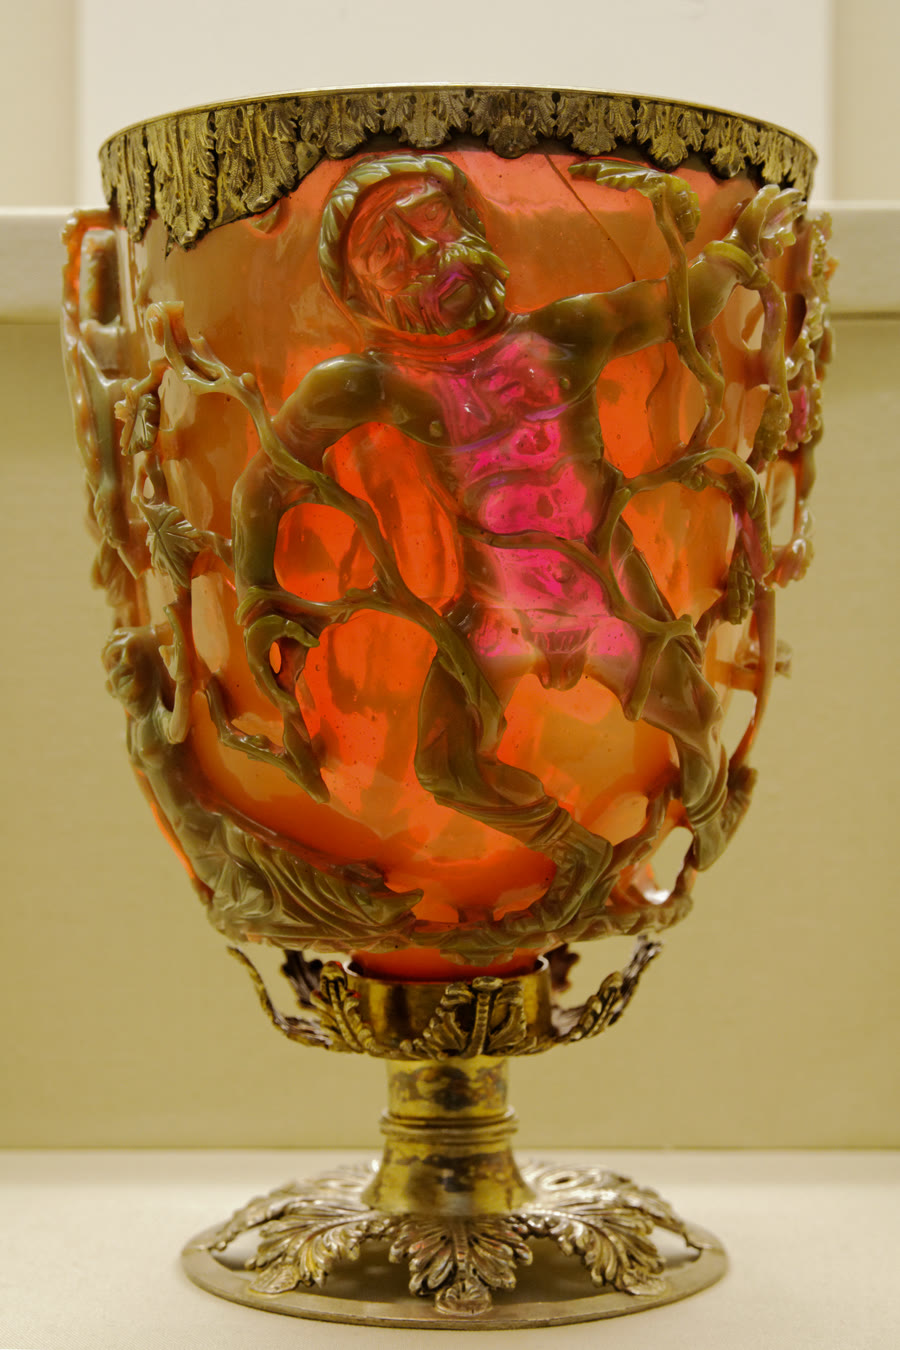
\includegraphics[width=0.32\linewidth]{images/book4/lycurgus-cup.jpg}

{\small Piala Lycurgus, sebuah benda kaca Romawi dari abad keempat, yang disinari dari dalam:
piala itu tampak hijau dalam cahaya pantul dan merah dalam cahaya terusan, sebuah efek
\omterm{def:b3:inorganic-materials:nano}{nanopartikel} emas--perak di dalam kaca. Foto: Marie-Lan Nguyen, CC BY
2.5.}
\end{omfigure}

\begin{history}[Nanopartikel sebelum ada katanya, dan bola sepak dari karbon]
Pembuat kaca mewarnai kaca menjadi merah dengan emas jauh sebelum orang tahu sebabnya;
piala Lycurgus memperlihatkan efek itu dalam bentuknya yang paling mencolok. Michael Faraday membuat
\omterm{def:b3:colloids:colloid}{koloid} emas pada tahun 1850-an dan melihat bahwa warnanya berasal dari partikel yang terlalu kecil
untuk dilihat. Pada 1985 Harold Kroto, Robert Curl, dan Richard Smalley, yang menguapkan
grafit dengan laser, mendapati bahwa gugusan enam puluh atom karbon
luar biasa stabil dan mengusulkan sangkar tertutup dengan dua belas segi lima dan
dua puluh segi enam; mereka menerima Hadiah Nobel Kimia 1996.
\end{history}

\section{Latihan}

\begin{exercise}[$\star$]\label{exo:b3:inorganic-materials:1}
Sebuah lapisan produk di antara dua padatan setebal \qty{2.0}{\micro\metre} setelah \qty{10}{h}. Berapa lama sampai lapisan itu
setebal \qty{6.0}{\micro\metre}, jika pertumbuhannya parabolik?
\end{exercise}

\begin{exercise}[$\star$]\label{exo:b3:inorganic-materials:2}
Tuliskan hidrolisis tetraetil ortosilikat menjadi asam silikat,
kondensasi dua molekul asam silikat, dan reaksi keseluruhan yang menghasilkan
silika.
\end{exercise}

\begin{exercise}[$\star$]\label{exo:b3:inorganic-materials:3}
Golongkan $\ce{SiO2}$, $\ce{B2O3}$, $\ce{Na2O}$, dan $\ce{CaO}$ sebagai pembentuk atau \omterm{def:b3:inorganic-materials:glass}{pengubah jaringan}, dan jelaskan apa yang
dilakukan $\ce{Na2O}$ pada jaringan silika.
\end{exercise}

\begin{exercise}[$\star$]\label{exo:b3:inorganic-materials:4}
Berapa banyak segi lima dan segi enam yang dimiliki $\ce{C70}$? Berapa banyak ikatannya?
\end{exercise}

\begin{exercise}[$\star\star$]\label{exo:b3:inorganic-materials:5}
% ledger: rion:Sr2+XII, rion:Ca2+XII, rion:Ba2+XII, rion:Ti4+VI, rion:O2-VI
Hitunglah \omterm{def:b3:inorganic-materials:perovskite}{faktor toleransi} $\ce{SrTiO3}$, $\ce{BaTiO3}$, dan $\ce{CaTiO3}$ dengan jari-jari berkoordinasi dua belas
$\ce{Sr^2+}$ (\qty{144}{pm}), $\ce{Ba^2+}$ (\qty{161}{pm}), dan $\ce{Ca^2+}$ (\qty{134}{pm}), $r(\ce{Ti^4+}) = \qty{60.5}{pm}$, dan $r(\ce{O^2-}) = \qty{140}{pm}$. Apakah
yang diramalkannya?
\end{exercise}

\begin{exercise}[$\star\star$]\label{exo:b3:inorganic-materials:6}
Sebuah \omterm{def:b3:inorganic-materials:zeolite}{zeolit} X memiliki rumus anhidrat $\mathrm{Na_{86}[(AlO_2)_{86}(SiO_2)_{106}]}$ (data latihan).
Berikan Si/Al dan kapasitas tukarnya untuk $\ce{Ca^2+}$ dalam milimol per gram.
\end{exercise}

\begin{exercise}[$\star\star$]\label{exo:b3:inorganic-materials:7}
% ledger: lat:Au
Emas berstruktur kubus berpusat muka dengan $a = \qty{407.8}{pm}$. Perkirakan jumlah kulit
partikel emas kuboktahedral yang berdiameter sekitar \qty{5}{nm}, jumlah atomnya, dan
fraksi atom di permukaannya.
\end{exercise}

\begin{exercise}[$\star\star$]\label{exo:b3:inorganic-materials:8}
Sebuah \omterm{def:b3:solid-state:classes}{semikonduktor} memiliki celah ruah \qty{1.74}{eV}, dan elektron serta \omterm{def:b3:solid-state:carriers}{lubangnya} memiliki \omterm{def:b3:quantum-model-systems:oscillator}{massa
tereduksi} $0.10\,m_e$ (data latihan). Perkirakan warna cahaya yang dipancarkan oleh
\omterm{def:b3:inorganic-materials:quantum-dot}{titik kuantum} berjari-jari 2.0 dan \qty{3.0}{nm}, dengan mengabaikan tarikan Coulomb.
\end{exercise}

\begin{exercise}[$\star\star$]\label{exo:b3:inorganic-materials:9}
Apakah nanotabung $(10, 10)$, $(10, 0)$, $(9, 0)$, dan $(12, 8)$ bersifat logam atau \omterm{def:b3:solid-state:classes}{semikonduktor}? Manakah
yang bertipe kursi, manakah yang zigzag?
\end{exercise}

\begin{exercise}[$\star\star\star$]\label{exo:b3:inorganic-materials:10}
% ledger: cod:MOF5.formula, cod:MOF5.a, cod:MOF5.Z
MOF-5, $\mathrm{Zn_4O(C_8H_4O_4)_3}$, berstruktur kubus dengan $a = \qty{25.82}{\angstrom}$ dan delapan satuan rumus per sel.
Hitunglah kerapatannya. Jika satu gram memiliki luas permukaan $\qty{3000}{m^2}$ (data
latihan), setara dengan berapa lapangan sepak bola berukuran $\qty{105}{m} \times \qty{68}{m}$ luas itu?
\end{exercise}

\begin{exercise}[$\star\star\star$]\label{exo:b3:inorganic-materials:11}
Dengan hitungan kulit pada \cref{prop:b3:inorganic-materials:magic}, tunjukkan bahwa
fraksi permukaan gugusan kuboktahedral menuju $3/n$ untuk $n$ yang besar, dan
bandingkan dengan fraksi eksak untuk $n = 8$.
\end{exercise}

\begin{exercise}[$\star\star\star$]\label{exo:b3:inorganic-materials:12}
Sebuah sangkar karbon tertutup dengan tiga ikatan per atom memuat $p$ segi lima, $h$ segi enam,
dan $s$ segi tujuh. Tunjukkan bahwa $p - s = 12$.
\end{exercise}

\section{Soal: Melunakkan Air dengan Zeolit A}

\begin{problem}[{Soal akhir pekan --- melunakkan air dengan zeolit A:
rumus dan aturan Löwenstein, kapasitas tukar teoretis, zeolit yang
diperlukan untuk satu kali cuci, dan jendela yang membiarkan kalsium masuk dan menahan deterjen
di luar}]
\label{pb:b3:inorganic-materials:1}
% ledger: iza:LTA.formula, iza:LTA.window, aw:Na, aw:Al, aw:Si, aw:O, aw:H, aw:Ca, aw:C, rion:Ca2+VI
\omterm{def:b3:inorganic-materials:zeolite}{Zeolit} A, yang dipakai dalam deterjen sebagai pengganti fosfat, memiliki rumus
$\mathrm{Na_{12}[(AlO_2)_{12}(SiO_2)_{12}]\cdot 27H_2O}$ dan jendela selebar \qty{0.41}{nm}. Sebuah air keran mengandung
\qty{2.0}{mmol/L} $\ce{Ca^2+}$, dan satu kali cuci memakai \qty{15}{L} air itu; dalam waktu satu kali cuci, \omterm{def:b3:inorganic-materials:zeolite}{zeolit} itu
mencapai 60\,\% kapasitasnya (data soal).

\medskip\noindent\textbf{Bagian I --- Rumus.}
\begin{enumerate}[beginpenalty=10000]
  \item Hitunglah massa molar rumus anhidratnya.
  \item Hitunglah massa molar rumus terhidratnya.
  \item Berikan Si/Al.
  \item Nyatakan aturan Löwenstein dan akibatnya di sini bagi susunan
        Si dan Al.
  \item Berapakah muatan kerangka per rumus?
  \item Hitunglah fraksi massa air dalam \omterm{def:b3:inorganic-materials:zeolite}{zeolit} terhidrat.
\end{enumerate}

\medskip\noindent\textbf{Bagian II --- Kapasitas tukar.}
\begin{enumerate}[resume, beginpenalty=10000]
  \item Tuliskan kesetimbangan pertukaran antara \omterm{def:b3:inorganic-materials:zeolite}{zeolit} natrium dan ion-ion
        kalsium.
  \item Berapa banyak $\ce{Ca^2+}$ yang dapat diambil oleh satu rumus?
  \item Hitunglah kapasitas teoretis \omterm{def:b3:inorganic-materials:zeolite}{zeolit} anhidrat dalam mmol $\ce{Ca^2+}$
        per gram.
  \item Hitunglah kapasitas itu untuk \omterm{def:b3:inorganic-materials:zeolite}{zeolit} terhidrat.
  \item Nyatakan kapasitas anhidrat sebagai miligram $\ce{CaCO3}$ per gram, yaitu satuan yang lazim
        untuk kesadahan air.
\end{enumerate}

\medskip\noindent\textbf{Bagian III --- Satu kali cuci.}
\begin{enumerate}[resume, beginpenalty=10000]
  \item Hitunglah jumlah $\ce{Ca^2+}$ dalam air satu kali cuci.
  \item Hitunglah massa \omterm{def:b3:inorganic-materials:zeolite}{zeolit} terhidrat yang diperlukan pada kapasitas teoretis.
  \item Hitunglah massa itu pada 60\,\% kapasitas.
  \item Hitunglah massa natrium yang dilepaskan ke dalam air.
  \item Mengapa produsen deterjen mengganti fosfat?
  \item Mengapa \omterm{def:b3:inorganic-materials:zeolite}{zeolit} A mengambil $\ce{Mg^2+}$ lebih lambat daripada $\ce{Ca^2+}$?
\end{enumerate}

\medskip\noindent\textbf{Bagian IV --- Jendela.}
\begin{enumerate}[resume, beginpenalty=10000]
  \item Bandingkan jendela itu dengan diameter ion $\ce{Ca^2+}$ (jari-jari berkoordinasi enam
        \qty{100}{pm}).
  \item Apakah yang harus dilakukan ion $\ce{Ca^2+}$ terhidrat agar dapat lewat?
  \item Mengapa anion \omterm{def:b3:colloids:surfactant}{surfaktan} seperti dodesil sulfat tetap di luar?
  \item Apakah fungsi \omterm{def:b3:inorganic-materials:zeolite}{zeolit} A sebagai zat pengering, dan mengapa \omterm{def:b3:inorganic-materials:zeolite}{zeolit} itu disebut
        \omterm{def:b3:inorganic-materials:zeolite}{ayakan molekul}?
  \item Bagaimana penggantian $\ce{Na+}$ dengan $\ce{K+}$ mengubah ukuran molekul yang diterima?
  \item Dalam ZSM-5, mengapa \textit{para}-xilena meninggalkan pori-pori lebih cepat daripada \textit{orto}-xilena?
  \item Nyatakan hasilnya: kapasitas tukar teoretis \omterm{def:b3:inorganic-materials:zeolite}{zeolit} A anhidrat
        untuk $\ce{Ca^2+}$.
\end{enumerate}
\end{problem}
